%\VignetteIndexEntry{Auckland child mortality 1977-1985 data set}
%\VignetteDepends{}
%\VignetteKeywords{spatial}
%\VignettePackage{spdep}
\documentclass[a4paper,10pt]{article} 
\usepackage{/usr/local/lib/R/share/texmf/Sweave}
\usepackage{times}
\usepackage{mathptm}
\usepackage{hyperref}
\setkeys{Gin}{width=0.95\textwidth}
\newcommand{\strong}[1]{{\normalfont\fontseries{b}\selectfont #1}}
\let\pkg=\strong
\RequirePackage{alltt}
\newenvironment{example}{\begin{alltt}}{\end{alltt}}
\newenvironment{smallexample}{\begin{alltt}\small}{\end{alltt}}
\newcommand{\code}[1]{\texttt{\small #1}}
\def\RR{\textsf{R}\/}
\def\SP{\texttt{S-PLUS}\/}
\def\SS{\texttt{S}\/}

\title{Auckland child mortality 1977-1985 data set} 
\author{Roger Bivand} 

\begin{document} 

\maketitle 




\section{Introduction}

Data on child mortalities for 167 census districts have been collected for a nine year period. Some census districts had very few cases, others larger numbers of cases. The underlying population at risk is taken as the 1981 census totals of children under 5. These data are only recorded for a single year, so need to be altered by a factor of nine to make them comparable to the mortality data. The data set is used by Marshall (1991), and presented in detail by Bailey and Gatrell (1995). It is their analysis we will be following here.

\begin{footnotesize}
\begin{Schunk}
\begin{Sinput}
> library(maptools)
> library(spdep)
\end{Sinput}
\begin{Soutput}
spdep, version 0.2-17, 2004-05-18:
 a package for analysing spatial dependence,
 use help(get.spChkOption) for help on integrity checking
\end{Soutput}
\begin{Sinput}
> data(auckland)
\end{Sinput}
\end{Schunk}
\end{footnotesize}

\section{Analysis of counts and proportions}

If the counts data were collected from census aggregates all having the same population of under-five children, the mortality rates (numbers per thousand per year) would already be standardised for variations in the sizes of the populations at risk. Since they are not --- as we can see from the summary of \code{Under.5.1981} in the \code{auckland} data frame, we need to standardise.


\begin{footnotesize}
\begin{Schunk}
\begin{Sinput}
> summary(auckland$Under.5.1981)
\end{Sinput}
\begin{Soutput}
   Min. 1st Qu.  Median    Mean 3rd Qu.    Max. 
    6.0   184.5   306.0   354.5   435.0  1407.0 
\end{Soutput}
\begin{Sinput}
> summary(auckland$Deaths.1977.85)
\end{Sinput}
\begin{Soutput}
   Min. 1st Qu.  Median    Mean 3rd Qu.    Max. 
  0.000   4.000   6.000   8.401  11.000  38.000 
\end{Soutput}
\begin{Sinput}
> res <- probmap(auckland$Deaths.1977.85, 9 * auckland$Under.5.1981)
> str(res)
\end{Sinput}
\begin{Soutput}
`data.frame':	167 obs. of  4 variables:
 $ raw     : num  0.00353 0.00494 0.00154 0.00243 0.00206 ...
 $ expCount: num  5.97 1.07 8.53 8.67 1.28 ...
 $ relRisk : num  133.9 187.5  58.6  92.2  78.1 ...
 $ pmap    : num  0.850 0.907 0.147 0.499 0.634 ...
\end{Soutput}
\end{Schunk}
\end{footnotesize}
The \code{probmap()} function provides four measures as columns of a data frame, when given a vector of counts $y_i$, and a vector of population at risk levels $n_i$. The first that we map (Figure \ref{raw}), using ``pretty'' class intervals, is for crude (raw) rates $r_i = y_i / n_i$, per thousand per year. 

\begin{footnotesize}
\begin{Schunk}
\begin{Sinput}
> brks <- c(-Inf, 2, 2.5, 3, 3.5, Inf)
> cols <- c("#F7F7F7", "#CCCCCC", "#969696", "#636363", "#252525")
\end{Sinput}
\end{Schunk}
\begin{Schunk}
\begin{Sinput}
> plot(auckpolys, col = cols[findInterval(res$raw * 1000, brks)], 
+     forcefill = FALSE)
> legend(c(70, 90), c(70, 95), fill = cols, legend = leglabs(brks), 
+     bty = "n")
\end{Sinput}
\end{Schunk}
\end{footnotesize}

\begin{figure}[htbp]
\begin{center} 
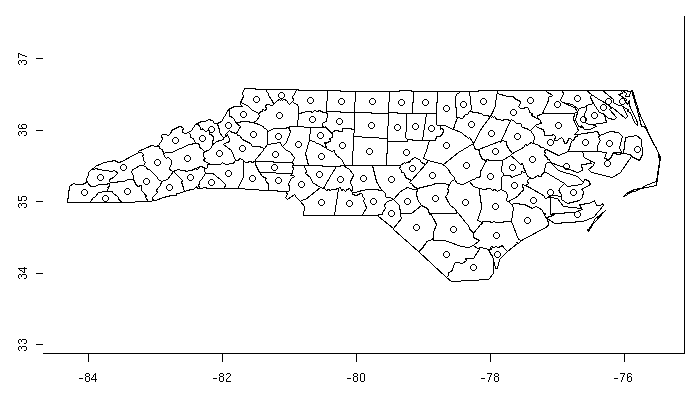
\includegraphics{Fig-bitmap-1.png}\end{center}
\caption{Crude (raw) estimates of infant mortality per 1000 per year, 1977--1985, Auckland}
\label{raw}
\end{figure}


\begin{footnotesize}
\begin{Schunk}
\begin{Sinput}
> brks <- c(-Inf, 47, 83, 118, 154, 190, Inf)
> cols <- c("#F7F7F7", "#CCCCCC", "#969696", "#636363", "#252525")
\end{Sinput}
\end{Schunk}
\begin{Schunk}
\begin{Sinput}
> plot(auckpolys, col = cols[findInterval(res$relRisk, brks)], 
+     forcefill = FALSE)
> legend(c(70, 90), c(70, 95), fill = cols, legend = leglabs(brks), 
+     bty = "n")
\end{Sinput}
\end{Schunk}
\end{footnotesize}
Next, we calculate the mean (expected) count as $\hat{\mu}_i = n_i ( \frac{\sum{y_i}}{\sum{n_i}})$, (Bailey and Gatrell p. 300). These values are also returned by the function, but not mapped here. Dividing the observed count in each census district by the expected count, and multiplying by 100, we get the standardised mortality rate, shown in Figure \ref{rel}; here the class intervals follow the book, Figure 8.1.

\begin{figure}[htbp]
\begin{center} 
\includegraphics{Fig-bitmap-2.png}\end{center}
\caption{Standardised mortality ratios for child deaths per year, 1977--1985, Auckland}
\label{rel}
\end{figure}


\begin{footnotesize}
\begin{Schunk}
\begin{Sinput}
> brks <- c(0, 0.05, 0.1, 0.2, 0.8, 0.9, 0.95, 1)
> cols <- c("#2166AC", "#67A9CF", "#D1E5F0", "#F7F7F7", "#FDDBC7", 
+     "#EF8A62", "#B2182B")
\end{Sinput}
\end{Schunk}
\begin{Schunk}
\begin{Sinput}
> plot(auckpolys, col = cols[findInterval(res$pmap, brks)], forcefill = FALSE)
> legend(c(70, 90), c(70, 95), fill = cols, legend = leglabs(brks), 
+     bty = "n")
\end{Sinput}
\end{Schunk}
\end{footnotesize}
Finally, we show a probability map in Figure \ref{pmap}. This is derived by passing the observed and expected counts as arguments to the \code{ppois()} distribution function for the Poisson distribution, and has two tails --- this differs from the derivation given by Bailey and Gatrell on p. 302. The values can be read as indicating how probable it is that a value as large as the observed count compared to the expected count could have arisen at random. Values close to zero indicate unusually small observed counts in relation to the expected counts, values close to unity indicate unusually large observed counts in relation to the expected counts.

\begin{figure}[htbp]
\begin{center} 
\includegraphics{Fig-bitmap-3.png}\end{center}
\caption{Poisson probabilities for child deaths per year, 1977--1985, Auckland}
\label{pmap}
\end{figure}

\section{Empirical Bayes estimates}

Section 8.2.2, pp. 303--308, describes in detail the background for calculating 
Empirical Bayes estimates of rates. Briefly, in census districts with small populations at risk, we place less weight on the local rate, and more on the global rate for all the districts considered together. 

\begin{footnotesize}
\begin{Schunk}
\begin{Sinput}
> res <- EBest(auckland$Deaths.1977.85, 9 * auckland$Under.5.1981)
\end{Sinput}
\end{Schunk}
\end{footnotesize}
Using the method of moments, the estimated values of the mean $\hat{\phi} = $ 7.2842e-07, and variance $\hat{\gamma} = $ 2.6334e-03 (returned as attributes of the data frame yielded by \code{EBest()}) correspond to those on p. 306. The mapped values (Figure \ref{EBest}) are essentially the same as Figure 8.3, but with the grey scale reversed, ``shrinking'' the rates of districts with small populations at risk towards the overall mean. 


\begin{footnotesize}
\begin{Schunk}
\begin{Sinput}
> brks <- c(-Inf, 2, 2.5, 3, 3.5, Inf)
> cols <- c("#F7F7F7", "#CCCCCC", "#969696", "#636363", "#252525")
\end{Sinput}
\end{Schunk}
\begin{Schunk}
\begin{Sinput}
> plot(auckpolys, col = cols[findInterval(res$estmm * 1000, brks)], 
+     forcefill = FALSE)
> legend(c(70, 90), c(70, 95), fill = cols, legend = leglabs(brks), 
+     bty = "n")
\end{Sinput}
\end{Schunk}
\end{footnotesize}

\begin{figure}[htbp]
\begin{center} 
\includegraphics{Fig-bitmap-4.png}\end{center}
\caption{Empirical Bayes global moment estimator of infant mortality per year, 1977--1985, Auckland}
\label{EBest}
\end{figure}


\section{Local Empirical Bayes estimates}

It is also possible, as Bailey and Gatrell indicate on p. 307, and in the exercises to the chapter on pp. 328--330, to ``shrink'' the estimates of census district rates not to the overall mean, but to neighbourhood means, where neighbourhoods are taken to be defined by districts sharing a boundary with the district of interest. Here, these shared boundaries have been listed in advance in the neighbours list object \code{auckland.nb}.

\begin{footnotesize}
\begin{Schunk}
\begin{Sinput}
> summary(auckland.nb)
\end{Sinput}
\begin{Soutput}
Neighbour list object:
Number of regions: 167 
Number of nonzero links: 772 
Percentage nonzero weights: 2.768116 
Average number of links: 4.622754 
Link number distribution:

 1  2  3  4  5  6  7  8  9 10 
 1  9 39 42 26 27 13  7  1  2 
1 least connected region:
128 with 1 link
2 most connected regions:
231 246 with 10 links
\end{Soutput}
\begin{Sinput}
> res <- EBlocal(spNamedVec("Deaths.1977.85", auckland), 9 * spNamedVec("Under.5.1981", 
+     auckland), auckland.nb)
\end{Sinput}
\end{Schunk}
\end{footnotesize}
As we can see, some neighbourhoods contain few districts, others relatively many. The idea is to ``shrink'' towards mean values that are appropriate for the part of the city that the district lies in, rather than to the overall mean value. On the other hand, the results will critically depend on our definition of neighbourhood.


\begin{footnotesize}
\begin{Schunk}
\begin{Sinput}
> brks <- c(-Inf, 2, 2.5, 3, 3.5, Inf)
> cols <- c("#F7F7F7", "#CCCCCC", "#969696", "#636363", "#252525")
\end{Sinput}
\end{Schunk}
\begin{Schunk}
\begin{Sinput}
> plot(auckpolys, col = cols[findInterval(res$est * 1000, brks)], 
+     forcefill = FALSE)
> legend(c(70, 90), c(70, 95), fill = cols, legend = leglabs(brks), 
+     bty = "n")
\end{Sinput}
\end{Schunk}
\end{footnotesize}
Figure \ref{EBloc} shows the results of the use of this function for the given definition of neighbours. You may like to compare the two Empirical Bayes estimates of the rates with the crude rates shown in Figure \ref{raw}. Do you still feel as confident as you did in the beginning about which census districts are reporting high rates?

\begin{figure}[htbp]
\begin{center} 
\includegraphics{Fig-bitmap-5.png}\end{center}
\caption{Empirical Bayes local moment estimator of infant mortality per year, 1977--1985, Auckland}
\label{EBloc}
\end{figure}

\section*{References}

\begin{description}

\item Marshall R M (1991) Mapping disease and mortality rates using
Empirical Bayes Estimators, \emph{Applied Statistics}, 40, 283--294.

\item Bailey T, Gatrell A (1995) \emph{Interactive Spatial Data Analysis},
Harlow: Longman.

\end{description}


\end{document}


